%!TEX root = ../Thesis.tex

\section{Computational scaling}\label{sec: Experimental work: Computational scaling}
%This section presents the parallel scaling capabilities of the \gls{VO} method as applied to both supervised and reinforcement learning problems.

\subsection{Scaling in supervised learning}
\begin{figure}[tbp!]
    \begin{subfigure}[b]{0.517\textwidth}
        \centering
        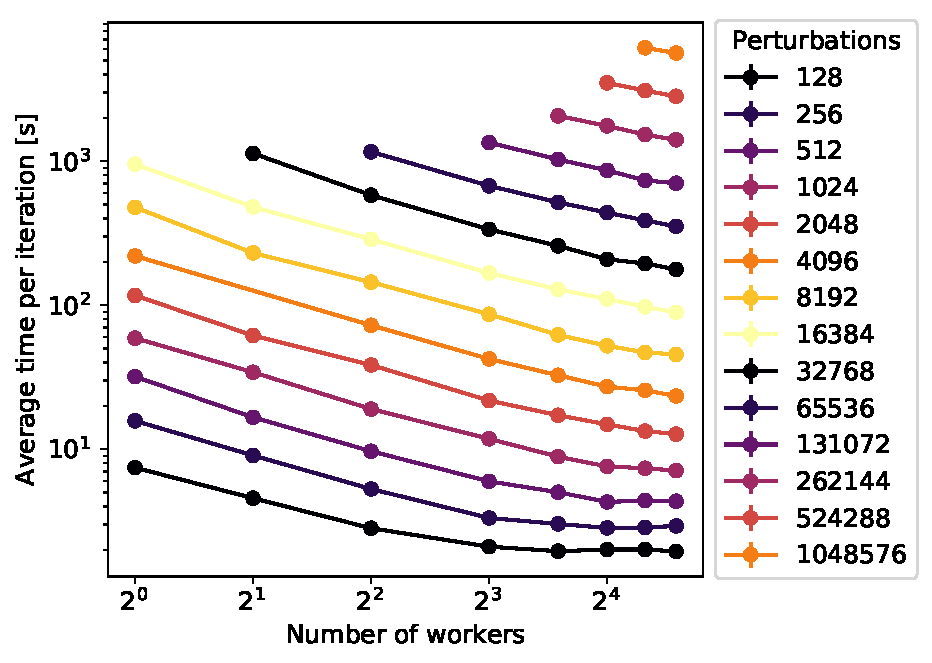
\includegraphics[height=5.6cm]{graphics/E005-sca-analysis/E005-scaling-02.pdf}
        \caption{}
        \label{fig: Theory: E005-scaling-supervised-02}
    \end{subfigure}
    \hfill
    \begin{subfigure}[b]{0.473\textwidth}
        \centering
        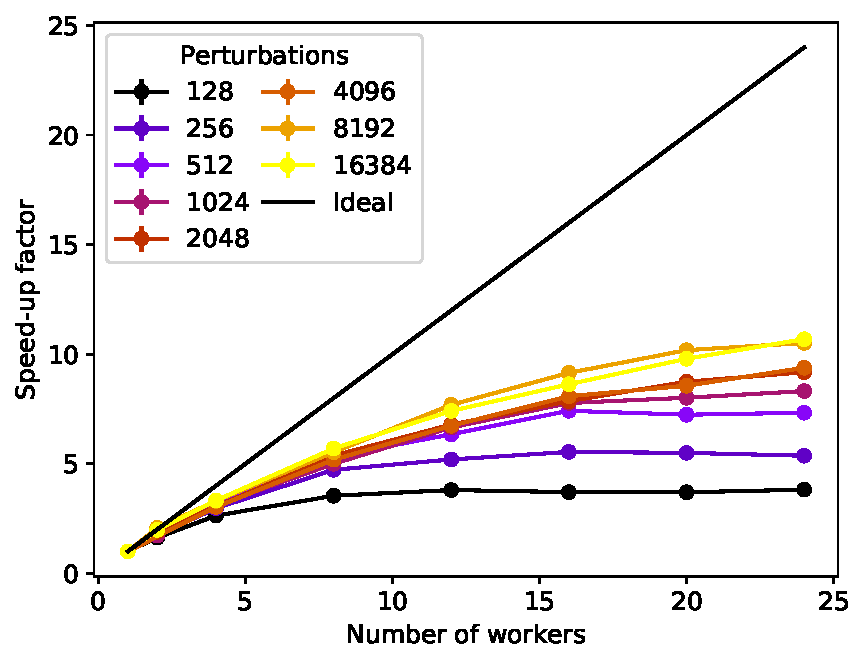
\includegraphics[height=5.6cm]{graphics/E005-sca-analysis/E005-scaling-04.pdf}
        \caption{}
        \label{fig: Theory: E005-scaling-supervised-04}
    \end{subfigure}
    \caption{
        Computational scaling in the supervised setting for different numbers of \glspl{CPU} and perturbations. Each observation is the average over 100 iterations with associated standard deviation (too small to discern).
        \subref{fig: Theory: E005-scaling-supervised-02} The average time spent per iteration in seconds.
        \subref{fig: Theory: E005-scaling-supervised-04} The observed speedup.
    }
    \label{fig: Theory: E005-scaling-supervised}
\end{figure}
This section presents the computational scaling of the \gls{VO} method used to train the \gls{MNIST} architecture described above when using a several \glspl{CPU} and varying the number of perturbations. 
Each setting of number of perturbations was run for 100 iterations and evaluated on a mini-batch of 200 images.
%Each perturbation was evaluated on a mini-batch of 200 images and each iteration of the algorithm evaluates some number of perturbations and was timed. 
The mean time and variance were computed from the 100 iterations run for each combination of number of \glspl{CPU} and perturbations.

\autoref{fig: Theory: E005-scaling-supervised-02} shows the average time spent per iteration as a function of the number of \glspl{CPU} used for various numbers of perturbations. The scaling can be seen to be fairly good for a high enough number of perturbations. Since the evaluation of every perturbation is a single forward pass through the network, the fitness evaluation is quite fast and slower function evaluations would give better scaling. \autoref{fig: Theory: E005-scaling-supervised-04} shows the measured speedup as a function of the number \glspl{CPU} for different perturbations. %This is a popular plot for presenting parallel performance and illustrates Amdahl's law \cite{Amdahl1967}. 
It is evident that speedup quickly drops off from the ideal although an order of magnitude speedup is observed for 24 \glspl{CPU}.

Obviously, \gls{VO} is an inefficient choice for optimizing differentiable \glspl{NN} in the supervised setting. Backpropagation excels at this task while also allowing for efficient batch parallelization on \glspl{GPU}.
%This points out the inefficiency of applying \gls{VO} to cases with relatively low cost fitness evaluations. Higher parallel
%Furthermore, this forward pass can be significantly sped up by using \glspl{GPU}.

\subsection{Scaling on a reinforcement learning problem}
\begin{figure}[tbp!]
    \begin{subfigure}[b]{0.504\textwidth}
        \centering
        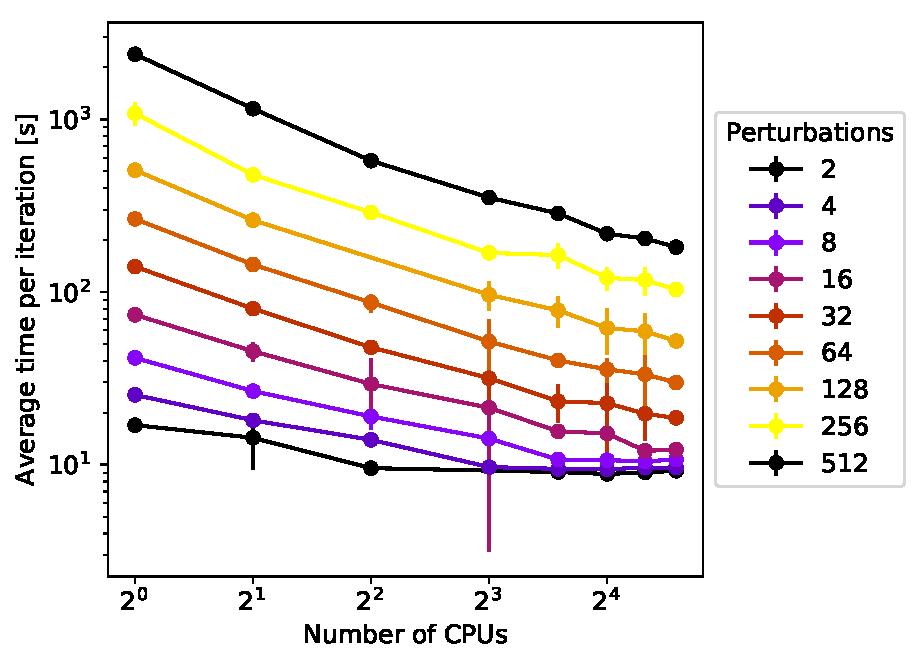
\includegraphics[height=5.7cm]{graphics/E011-sca-analysis/E011-scaling-02.pdf}
        \caption{}
        \label{fig: Theory: E011-scaling-supervised-02}
    \end{subfigure}
    \hfill
    \begin{subfigure}[b]{0.486\textwidth}
        \centering
        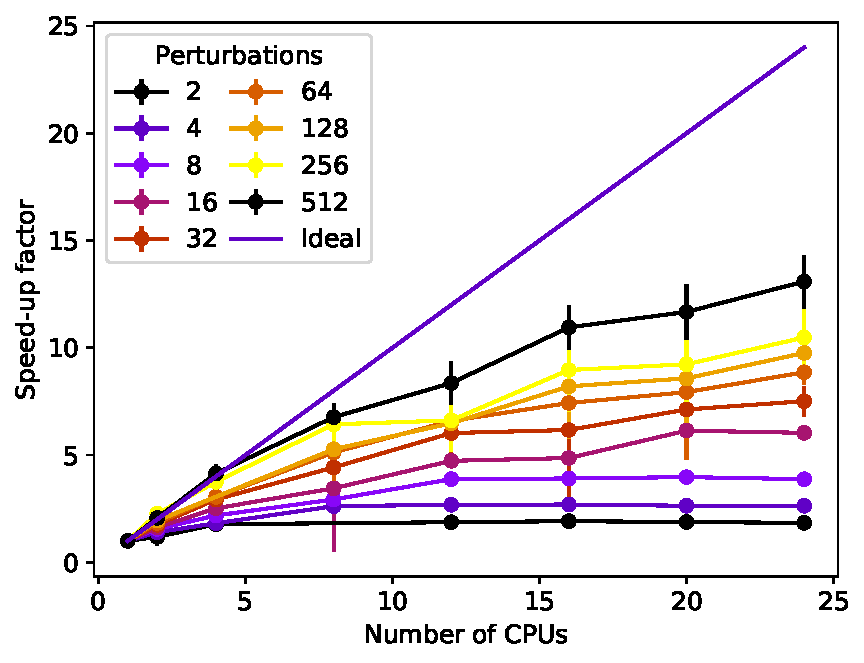
\includegraphics[height=5.7cm]{graphics/E011-sca-analysis/E011-scaling-04.pdf}
        \caption{}
        \label{fig: Theory: E011-scaling-supervised-04}
    \end{subfigure}
    \caption{
        Computational scaling in the reinforcement learning setting for different numbers of \glspl{CPU} and perturbations. Each observation is the average over 100 iterations with associated standard deviation.
        \subref{fig: Theory: E011-scaling-supervised-02} The average time spent per iteration in seconds.
        \subref{fig: Theory: E011-scaling-supervised-04} The observed speedup.
    }
    \label{fig: Theory: E011-scaling-supervised}
\end{figure}

This section presents the results of running the same scaling experiment as before but here on the Atari-2600 game Freeway. The used network is the DQN from \cite{Mnih2015} and preprocessing is as described above. Each episode was limited to 1000 frames (episode horizon) and 100 episodes were simulated for each combination of number of \glspl{CPU} and perturbations. Freeway was chosen since it has a fixed episode duration allowing the use of untrained policies in the experiment. This removes the dependency of the scaling on the quality of the policy.

The results are presented in the same form as for the supervised case in \autoref{fig: Theory: E011-scaling-supervised}. The scaling is somewhat better than for the supervised case and it is achieved for much lower numbers of perturbations as a result of the much more expensive fitness evaluation. For 512 perturbations, increasing the number of \glspl{CPU} from 1 to 4 provides an almost monomial decrease in the time spent per iteration. This is as observed in \cite{Salimans2017} although the computational resources expended for experimentation were much greater than here. Conclusively, reinforcement learning is much more well suited for the \gls{VO} method supervised learning.
%Here, the fitness function evaluation relies on simulation of some often complex environment and the required forward passes of the policy network are inherently sequential.